This chapter presents the design decisions taken while implementing \acrfull{wdias}, and how is the system got \hl{adapted from the systems analyzed in Chapter} \ref{ch:literature}.
\cref{se:high_level_design} presents a brief discussion on how the weather forecasting is happening and why it needs to interact with multiple data formats.
\cref{se:architectural_decisions} presents how the architectural design of proposed solution evolved while designing and implementing \acrshort{wdias}.
\cref{se:microservice} presents %gives a better understanding of the 
microservice architectural concepts followed while implementing \acrshort{wdias}.
Then the reasons behind developing \acrshort{wdias} database structure and technologies used are discussed in \cref{se:db_struct}.
\cref{se:data_preprocess} discusses how \acrshort{wdias} enables data preprocessing and adding capabilities using extensions.
Finally, \cref{se:query} includes details on how to perform timeseries search and geo-based queries on the \acrshort{wdias}.

\dbc{It's just WDIAS. "the" should be used only on essential places to being the meaning. }
%%%%%%%%%%%%%%%%%%%%%%%%%%%%%%%%%%%%%%%%%%%%%%%%%%%%%%%%%%%%%%%%%%%%%%%%%%%%%%%%
\section{High-level Design}
\label{se:high_level_design}

To get an overall idea of the flow of weather prediction, let us look into one of the \hl{flows using} at the \acrshort{curw} \cite{CUrWSL2017SL}.

\begin{enumerate}
    \item Extract \acrshort{GRIB} \acrshort{wrf} model data to \acrshort{netCDF}
    \item \hl{From} \acrshort{netCDF} to \acrshort{csv} of each location data, then feed to HEC-HMS hydro-dynamic model and get the output as a \acrshort{csv} file.
    \item \acrshort{csv} and \hl{Rain cell Grid feed} into the FLO2D hydrologic model, and get the water level as ASCII Grid files after the simulation is complete.
    \item Upload ASCII files to \hl{ArcGIS create raster files, then use for the LOSS Estimation}
\end{enumerate}

\hl{When looked into the above flow, it gives a clear understanding of multiple data formats using while weather predictions.}
Also, to correct the model outputs, \hl{it required} to collect real-time data such as:
\begin{itemize}
    \item Frequently collected automated weather station data via HTTP protocol
    \item Frequently collected automated water level stations data
\end{itemize}

\hl{Other than above many data formats using for handling data based on devices and standards which are using.} Also, for data modeling, it needs to convert the data \hl{into model compatible data format}. Then \hl{after successfully run the model it needs to collect data from the model output data formats.}

%%%%%%%%%%%%%%%%%%%%%%%%%%%%%%%%%%%%%%%%%%%%%%%%%%%%%%%%%%%%%%%%%
\subsection{Modules of a Weather Data System}
\label{subse:modules_weather_data_integration_sys}

\cref{fi:wdia_components} shows the basic functions of a weather data integration and assimilation system consisting of the following modules:

\begin{figure}[htbp]
\centerline{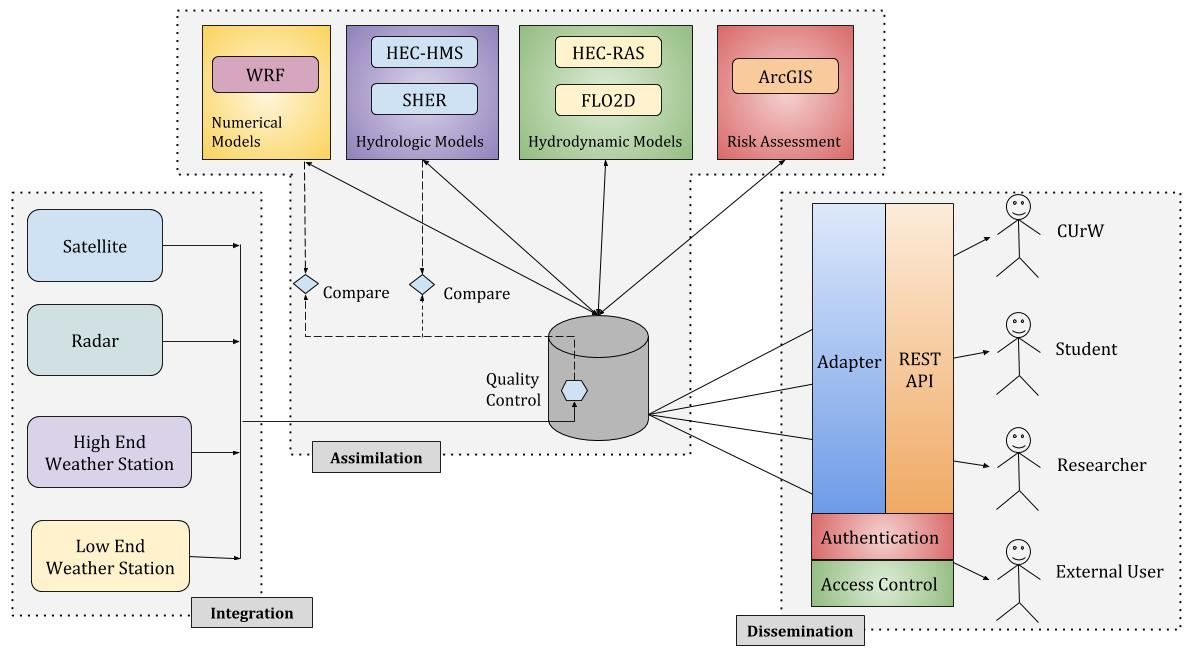
\includegraphics[width=1\textwidth]{method/misc/weather_data_system_components.jpg}}
\caption{Modules of a weather data system.}
\label{fi:wdia_components}
\end{figure}

\subsubsection{Integration}
The system should capable of integrating data from different sources such as satellite data, high end, and low-end weather station, etc. And the system should be able to handle multidimensional spatial and temporal weather data efficiently and optimally. 
\subsubsection{Assimilation}
Then the system should be able to fulfill weather models varying data requirements. Also, those models reproduce a large set of redundant data, thus the system should store the bulk data while optimizing the disk space.
\subsubsection{Dissemination}
Then different users should be able to retrieve data as they required. Also, the users should be able to easy to search into the available that in the system base on timeseries metadata or based on Geo queries.


%%%%%%%%%%%%%%%%%%%%%%%%%%%%%%%%%%%%%%%%%%%%%%%%%%%%%%%%%%%%%%%%%%%%%%%%%%%%%%%%

% \paragraph{Timeseries}-- A timeseries is simply a series of data points ordered in time. In weather domain, it interest in timeseries in perspective of observations to forecasting. Each timeseries, the data points can be form in different formats as well. For example, scalar (0D), vector (1D), grid (2D), and polygon (2D).

% In the proof of concept design described below, WDIAS focuses on handling scalar, vector and grid timeseries data. However, the system could be extended to handle polygon-based timeseries as well.

% \subsubsection{Base of WDIAS architecture}
% \hl{The base of WDIAS architecture origins based on attributes of a timeseries.} There are many attributes to differentiate timeseries one from another. But 
% Among many attribute to differentiate a timeseries from another, the following can be consider as the key attributes in uniquely identify a timeseries from another: % for the \acrshort{wdias}.

% \begin{itemize}
%     \item Module -- module that generates the timeseries
%     \item Value type -- Scalar, vector, grid, or polygon
%     \item Location of readings
%     \item Parameter -- measuared parameter
%     \item hl{Timeseries type}
%     \begin{itemize}
%         \item Sources -- External or simulated
%         \item Category -- Historical or forecast
%     \end{itemize}
%     \item Time step
% \end{itemize}
% \dbc{Use bullets only when essential. Other places use paragraphs.}

% A detail description of the above attributes are presented in \cref{se:db_struct}.